Juana arma triángulos con fósforos. Arma figuras que guardan una relación en particular. Observa la siguiente imagen:

\begin{minipage}{0.4\linewidth}
    \begin{figure}[H]
        \centering
        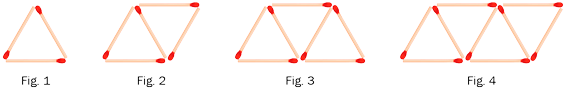
\includegraphics[width=0.9\linewidth]{../images/c9b918ae22f368bf3b8bbb644dfd20d4530338f0}
    \end{figure}
\end{minipage}\hfill
\begin{minipage}{0.6\linewidth}
    Juana sigue armando triángulos según la secuencia de la imagen.
    Cuando termine de armar la Fig 25,
    \textbf{¿cuántos fósforos habrá usado en total?}\\
\end{minipage}

\begin{solutionbox}{4cm}
    Ya que la regla de recurrencia es:
    \[a_n=2(n-1)+3\]
    entonces,
    \[a_{25}=2(25-1)+3=48+3=51\]
    y,
    \[s_{25}=\dfrac{25(a_0+a_{25})}{2}=\dfrac{25(3+51)}{2}=675\]\end{solutionbox}
